\chapter{Datensatz und Datenvorbereitung}
\label{chap:datensatz}

Dieses Kapitel legt die Grundlage der experimentellen Evaluation. Es ordnet die Datensätze DDoS-AT-2022 und IoT-DH ein, beschreibt die Datenvorverarbeitung und Merkmalsstruktur und erläutert das Flussmodell, aus dem die Experimentdaten entstehen. Die Qualität der Datengrundlage ist in der Erkennung von Netzwerkangriffen von zentraler Bedeutung, da bereits kleine Unterschiede in der Datenrepräsentation, der Labelgenauigkeit oder der zeitlichen Aggregation die Leistungsfähigkeit eines Klassifikators maßgeblich beeinflussen können. Vor diesem Hintergrund werden im Folgenden die verwendeten Evaluationsdatensätze, die Vorverarbeitungsschritte, die Feature-Extraktion, das Generatormodell der Experimentdaten und die Maßnahmen zur Berücksichtigung von Klassenungleichgewichten beschrieben.

\section{Verwendete Evaluationsdatensätze}
\label{sec:datensaetze}

Die Aufgabenstellung verlangt einen Datensatz, der Netzverkehr mit einem DDoS-Angriff beschreibt. Für die Auswahl gelten drei Kriterien. Der Datensatz muss legitimen Verkehr und Angriffsverkehr mit eindeutigen Labels enthalten. Er muss in einer Veröffentlichung dokumentiert sein, die Merkmale, Erfassungsmethodik und Angriffsarten beschreibt. Und seine Merkmale müssen flussbasiert sein, damit sie sich als Zustandsvektor eines Agenten abbilden lassen. Zwei öffentlich dokumentierte Datensätze erfüllen diese Kriterien und decken zwei unterschiedliche Netzumgebungen ab.

\subsection*{DDoS-AT-2022}

Mittal et al. erzeugen DDoS-AT-2022 in einem selbst entworfenen DDoS-Testbed auf Basis des CORE-Emulators \autocite{mittalDDoSAT2022DistributedDenial2023}. Der Datensatz ist emulationsbasiert und mischt legitimen Verkehr, Flash-Traffic und verschiedene DDoS-Angriffe auf Transport- und Anwendungsschicht, jeweils mit unterschiedlichen Angriffsraten (low, slow, flood). Zu den Transportschicht-Angriffen zählen UDP-Flood sowie TCP-Angriffe vom Typ SYN, ACK, RST und FIN, zu den Anwendungsschicht-Angriffen langsame HTTP-Varianten wie Slow Body, Slow Read und Slow Header. Die Autoren extrahieren die Flussmerkmale mit CICFlowMeter und labeln den Verkehr anschließend. Ihr Argument für den neuen Datensatz lautet, dass vorhandene Datensätze entweder simuliert sind oder keine ausgewogene Mischung verschiedener Angriffstypen und Angriffsraten enthalten. Die Mischung aus Flash-Traffic und Angriffsverkehr ist für diese Arbeit besonders relevant, weil sie die Überlappung von legitimem Lastanstieg und Angriff abbildet, die auch das Generatormodell in Abschnitt~\ref{sec:generatormodell} nachbildet.

\subsection*{IoT-DH}

IoT-DH von Saif et al. stammt aus einer Honeypot-Umgebung für IoT-Geräte (RIoTPot), deren Verkehr als PCAP aufgezeichnet und in CSV überführt wurde \autocite{saifIoTDHDatasetClassification2024}. Der Datensatz enthält zehn Merkmale, darunter die Paketankunftsrate (\texttt{pktrate}), die Dauer zwischen aufeinanderfolgenden Paketen (\texttt{dt}, \texttt{dur}), das Protokoll, die Portnummer und die übertragenen und empfangenen Datenraten in kbit/s (\texttt{tx\_kbps}, \texttt{rx\_kbps}, \texttt{tot\_kbps}). Das Label ist binär (0 normal, 1 Angriff). In der Erprobung durch die Autoren erreicht ein Random Forest auf 10\,000 Einträgen mit 80\,\%/20\,\%-Split eine Genauigkeit von 98\,\%, im Testsplit sind 748 von 2000 Einträgen Angriffe, also rund 37\,\%.

\subsection*{Einordnung für die vorliegende Arbeit}

Beide Datensätze ergänzen sich. DDoS-AT-2022 liefert einen Verkehr mit vielfältigen Angriffstypen und Raten in einem emulierten Netz, IoT-DH Datenraten und Paketzeiten aus einer IoT-Umgebung, in der vor allem schwache Geräte betroffen sind \autocite{balaAITechniquesIoTbased2024}. Beide enthalten flussbasierte Merkmale, deren Gruppen (Paketrate, Datenrate, Zeitabstände, Protokollanteile) die Merkmalsstruktur in Abschnitt~\ref{sec:feature_extraktion} motivieren. Die Experimente in Kapitel~\ref{chap:evaluierung} verwenden die Rohdaten beider Datensätze nicht direkt. Stattdessen erzeugt ein parametrisches Flussmodell (Abschnitt~\ref{sec:generatormodell}) Merkmalsvektoren, deren Struktur sich an diesen Datensätzen orientiert. Das erlaubt es, den SNR kontrolliert zu variieren und die Klassenüberlappung exakt festzulegen. Es bedeutet aber auch, dass die berichteten Kennzahlen nicht ohne Weiteres auf die Originaldaten übertragbar sind. Der Nachweis an den Originaldatensätzen bleibt ein Schritt, den Kapitel~\ref{chap:fazit} als Ausblick aufgreift.

\section{Datenvorverarbeitung}
\label{sec:datenvorverarbeitung}

Die Rohdaten aus Netzwerk- und Angriffsdatensätzen liegen in der Regel nicht direkt im für maschinelles Lernen optimierten Format vor. Sie enthalten häufig redundante Informationen, inkonsistente Einträge, fehlende Werte, verteilte Zeitstempel oder unterschiedliche Skalenniveaus zwischen numerischen und kategorialen Attributen. Aus diesem Grund ist eine systematische Datenvorverarbeitung ein zentraler Bestandteil der Pipeline, da sie die Erkennbarkeit relevanter Muster verbessert und die Stabilität des Lernprozesses erhöht. Die Vorverarbeitung umfasst daher typischerweise das Bereinigen der Daten, die Harmonisierung der Datentypen, die Behandlung fehlender Werte, die Normalisierung numerischer Merkmale und die Transformation von kategorialen Informationen in maschinell verarbeitbare Repräsentationen.

Im ersten Verarbeitungsschritt werden die Rohdaten importiert und strukturiert analysiert. Dabei werden Informationen wie Zeitstempel, Protokolltypen, Source- und Destination-Attribute, Paketgrößen, Verbindungsdauer und Flag-Informationen mit den zugehörigen Labels abgeglichen. Anschließend werden fehlerhafte, doppelte oder nicht interpretierbare Einträge identifiziert und entsprechend behandelt. Dies ist insbesondere bei Netzwerkdaten von Bedeutung, da unvollständige oder inkonsistente Aufzeichnungen durch Messfehler, fehlende Paketinformationen oder unterschiedliche Messquellen entstehen können. Eine sorgfältige Bereinigung verhindert, dass das Modell durch verrauschte oder fehlerhafte Eingaben systematisch verzerrt wird.

In einem weiteren Schritt werden die Merkmalswerte in ein einheitliches Format überführt. Numerische Attribute wie Paketanzahlen, Flussdauer oder Interarrival-Zeiten werden häufig skaliert, um Unterschiede in der Maßstabsebene zu berücksichtigen und die Optimierung der Lernalgorithmen zu stabilisieren. Kategoriale Attribute wie Protokolltypen, Dienstnamen oder Zustandsinformationen werden in numerische Repräsentationen transformiert, was je nach Modelltyp durch One-Hot-Encoding, ordinales Encoding oder andere geeignete Verfahren erfolgen kann. Zudem werden zeitliche Zusammenhänge durch Aggregation auf Fluss- oder Zeitfensterebene modelliert, damit relevante Verkehrsmuster auch bei hochdimensionalem Datenstrom erkennbar bleiben.

Ein weiterer wichtiger Bestandteil der Datenvorverarbeitung ist die Aufteilung der Daten in unabhängige Mengen für Training und Test. Die Trennung muss so erfolgen, dass keine Informationslecks zwischen den Teilmengen entstehen und die spätere Leistungsbewertung auf tatsächlich unbekannten Daten basiert. In einem sicherheitsrelevanten Kontext ist dies besonders kritisch, da zeitliche Abhängigkeiten und ähnliche Verkehrsprofile sonst künstlich zu hohe Werte für Genauigkeit und Generalisierung erzeugen können. Die Vorverarbeitung bildet somit nicht nur eine technische Vorbereitung, sondern zugleich eine methodische Garantiestruktur für die Validität der experimentellen Ergebnisse.

\section{Feature-Extraktion}
\label{sec:feature_extraktion}

Die Feature-Extraktion stellt den Übergang von den Rohdaten zu einer lernbaren Repräsentation des Netzwerkverkehrs dar. Während in der ursprünglichen Logdatei oder im Paketstrom häufig eine Vielzahl semantisch komplexer Informationen enthalten ist, wird für maschinelle Lernverfahren eine abstrahierte Merkmalsmenge benötigt, die relevante Unterschiede zwischen normalem und anomalem Verhalten widerspiegelt. In der DDoS-Erkennung sind insbesondere Merkmale relevant, die das Verkehrsvolumen, die Paketstruktur, die zeitliche Dynamik und das Netzwerkverhalten eines Flusses oder einer Verbindung charakterisieren. Damit bildet die Feature-Auswahl eine entscheidende Voraussetzung für die Modellgüte und die Interpretierbarkeit der Ergebnisse.

Die in den Datensätzen und in der Literatur verwendeten Merkmale lassen sich in verschiedene Gruppen einteilen. Zu den volumetrischen Kennzahlen zählen beispielsweise Paketanzahlen, Bytevolumen, Flussgrößen und Verbindungsraten, die Aufschluss über die Intensität des Datenverkehrs geben. Zeitliche Merkmale wie Interarrival-Zeiten, Flussdauer, Dauer von Burst-Phasen oder statistische Verteilungen über Zeitfenster erfassen dynamische Muster und können besonders bei langsam ansteigenden oder zeitlich gestaffelten Angriffen relevant sein. Protokoll- und Verbindungsmerkmale, etwa TCP-/UDP-Anteil, Portnutzung, Zustandscodes und Verbindungstypen, helfen dabei, typische Kommunikationsmuster von legitimen und bösartigen Strömen zu unterscheiden. Ergänzend können statistische Aggregationen wie Mittelwert, Varianz, Median oder Quantile über Zeitfenster verwendet werden, um robuste Indikatoren für Anomalien zu erzeugen.

Die Auswahl und Gestaltung der Features erfolgt dabei nicht aus rein technischer Notwendigkeit, sondern auf Basis des zugrunde liegenden Angriffsbildes. Ein DDoS-Angriff manifestiert sich typischerweise in einer starken Veränderung der Kommunikationsparameter, etwa durch erhöhte Paketfrequenz, abnormalen Ressourcenverbrauch oder ungewöhnliche Verteilungsstrukturen zwischen Clients und Servern. Die Feature-Extraktion soll deshalb genau jene Charakteristika erfassen, die sich zwischen legitimem und aggressivem Verkehr unterscheiden. Gleichzeitig ist die Dimensionierung der Merkmale kritisch, da sowohl eine zu geringe Repräsentation als auch eine zu hohe Dimensionalität die Lernfähigkeit und Generalisierung des Modells beeinträchtigen können.

Nach der Extraktion werden die Merkmale weiter auf ihre Informationsgehalt, Konsistenz und Robustheit überprüft. Merkmale mit geringer Varianz, hoher Korrelation oder fehlender Aussagekraft für die Zielklasse können entfernt oder zusammengefasst werden, um die Lernaufgabe zu vereinfachen und Overfitting zu vermeiden. In der praktischen Umsetzung bildet diese Auswahlphase daher eine Verbindung zwischen domänenwissenbasierten Annahmen und datengetriebenen Optimierungsprozessen. Sie ist entscheidend für die spätere Modellleistung und die interpretierbare Bewertung des erkannten Angriffsverhaltens.

\section{Generatormodell der Evaluationsdaten}
\label{sec:generatormodell}

Für die kontrollierten SNR-Experimente beschreibt jeder Netzwerkfluss ein Vektor $\mathbf{x}\in\mathbb{R}^{8}$ aus acht normierten Merkmalen. Sie stehen stellvertretend für die in Abschnitt~\ref{sec:feature_extraktion} genannten Gruppen, etwa Paketrate, SYN-Anteil oder die Entropie der Quelladressen, wie sie in den Datensätzen \autocite{mittalDDoSAT2022DistributedDenial2023, saifIoTDHDatasetClassification2024} und in der Merkmalsauswahl von Raza et al. \autocite{razaFeatureSelectionBasedDDoSAttack2024} auftreten. Das Modell ist klassenbedingt gaußverteilt:
\begin{equation}
	\mathbf{x}\mid c \sim \mathcal{N}\!\left(\boldsymbol{\mu}_c,\ \sigma^2\mathbf{I}\right),\qquad c\in\{\text{Normal},\text{DDoS}\},\quad \sigma=0{,}20 .
\end{equation}
Die Klassenmittelwerte unterscheiden sich je Merkmal nur um $0{,}15$ bis $0{,}25$ und liegen damit im Bereich der Streuung $\sigma$. Die Klassen überlappen also bewusst, so wie legitimer Lastanstieg und niederratige Angriffe in realen Datensätzen \autocite{mittalDDoSAT2022DistributedDenial2023}. Der Angriffsanteil beträgt $\pi=0{,}3$. Das liegt in der Größenordnung der 37\,\% Angriffsanteil im Testsplit von IoT-DH und bildet das für Sicherheitsanwendungen typische Klassenungleichgewicht ab \autocite{saifIoTDHDatasetClassification2024}.

Der Agent beobachtet nicht $\mathbf{x}$, sondern die über einen AWGN-Kanal gestörte Version $\mathbf{y}=\mathbf{x}+\mathbf{n}$ mit unabhängigen Rauschtermen $n_j\sim\mathcal{N}(0,\sigma_{n,j}^2)$. Die Rauschvarianz folgt aus der Signalleistung $P_j=\mathbb{E}[x_j^2]$ des Merkmals $j$ (Mischung beider Klassen) und dem SNR:
\begin{equation}
	\sigma_{n,j}^2=\frac{P_j}{10^{\mathrm{SNR_{dB}}/10}},\qquad P_j=(1-\pi)\,\mu_{\text{Normal},j}^2+\pi\,\mu_{\text{DDoS},j}^2+\sigma^2 .
\end{equation}
Abbildung~\ref{fig:generator_ablauf} fasst den Ablauf zusammen und zeigt am Merkmal $j=1$ ($\mu_{\text{Normal},1}=0{,}30$, $\mu_{\text{DDoS},1}=0{,}55$), wie das Rauschen die Klassendichten verbreitert. Bei $30$\,dB bleibt $\sigma_{n,1}\approx0{,}015$ neben $\sigma=0{,}20$ unerheblich, bei $5$\,dB wächst die effektive Streuung auf $\sqrt{\sigma^2+\sigma_{n,1}^2}\approx0{,}34$ und die Dichten überdecken einander weitgehend.

\begin{figure}[htbp]
	\centering
	\begin{tikzpicture}[
		font=\small,
		blk/.style={draw, rectangle, rounded corners=2pt, minimum height=1.6cm, text width=3.3cm, align=center, thick},
		arr/.style={-{Stealth[length=2.2mm]}, thick},
		node distance=0.6cm
	]
		\node[blk] (lab) {Label ziehen\\ $c\sim\mathrm{Bern}(\pi)$, $\pi=0{,}3$};
		\node[blk, right=of lab] (gau) {Gauß-Merkmale\\ $\mathbf{x}\sim\mathcal{N}(\boldsymbol\mu_c,\sigma^2\mathbf{I})$, $\sigma=0{,}20$};
		\node[blk, right=of gau, fill=blue!8] (aw) {AWGN\\ $\mathbf{y}=\mathbf{x}+\mathbf{n}$, $\sigma_{n,j}^2=\dfrac{P_j}{10^{\mathrm{SNR}/10}}$};
		\draw[arr] (lab) -- node[above, font=\scriptsize] {$c$} (gau);
		\draw[arr] (gau) -- node[above, font=\scriptsize] {$\mathbf{x}$} (aw);
		\node[above=0.35cm of aw, font=\scriptsize] (snr) {SNR $\in\{30,20,10,5\}$\,dB};
		\draw[arr] (snr) -- (aw);

		% Dichtediagramme
		\begin{scope}[shift={(0,-5.6)}, xscale=2.2, yscale=0.9]
			\draw[->] (-0.5,0) -- (1.35,0) node[right, font=\scriptsize] {$y_1$};
			\draw[->] (-0.5,0) -- (-0.5,2.3);
			\draw[thick, blue!70!black, domain=-0.5:1.3, samples=70] plot (\x, {1.99*exp(-((\x-0.30)^2)/(2*0.0402))});
			\draw[thick, red!70!black, domain=-0.5:1.3, samples=70] plot (\x, {1.99*exp(-((\x-0.55)^2)/(2*0.0402))});
			\draw[dotted] (0.30,0) -- (0.30,2.0);
			\draw[dotted] (0.55,0) -- (0.55,2.0);
			\node[font=\scriptsize] at (0.1,-0.45) {$\mu_{\text{N}}=0{,}30$};
			\node[font=\scriptsize] at (0.78,-0.45) {$\mu_{\text{A}}=0{,}55$};
			\node[font=\scriptsize, align=center] at (0.43,2.65) {(a) $30$\,dB: $\sigma_{\mathrm{eff}}\approx0{,}20$};
		\end{scope}
		\begin{scope}[shift={(7.6,-5.6)}, xscale=2.2, yscale=0.9]
			\draw[->] (-0.5,0) -- (1.35,0) node[right, font=\scriptsize] {$y_1$};
			\draw[->] (-0.5,0) -- (-0.5,2.3);
			\draw[thick, blue!70!black, domain=-0.5:1.3, samples=70] plot (\x, {1.18*exp(-((\x-0.30)^2)/(2*0.1137))});
			\draw[thick, red!70!black, domain=-0.5:1.3, samples=70] plot (\x, {1.18*exp(-((\x-0.55)^2)/(2*0.1137))});
			\draw[dotted] (0.30,0) -- (0.30,1.2);
			\draw[dotted] (0.55,0) -- (0.55,1.2);
			\node[font=\scriptsize] at (0.1,-0.45) {$\mu_{\text{N}}$};
			\node[font=\scriptsize] at (0.78,-0.45) {$\mu_{\text{A}}$};
			\node[font=\scriptsize, align=center] at (0.43,2.65) {(b) $5$\,dB: $\sigma_{\mathrm{eff}}\approx0{,}34$};
		\end{scope}
	\end{tikzpicture}
	\caption{Datengenerator mit AWGN-Kanal. Oben: Ablauf von Label, Gauß-Merkmalen und Rauschen. Unten: Klassenbedingte Dichten (blau: Normal, rot: DDoS) des Merkmals $y_1$ bei (a) hohem und (b) niedrigem SNR. Die Mittelwerte bleiben fest, nur die Streuung wächst.}
	\label{fig:generator_ablauf}
\end{figure}

Abbildung~\ref{fig:feature_raum_3d} zeigt dieselben $1\,500$ Flüsse im Teilraum der Merkmale $y_1$, $y_2$ und $y_4$, einmal bei $30$\,dB und einmal bei $5$\,dB. Bei $30$\,dB bilden Normal- und DDoS-Verkehr zwei erkennbare, wenn auch bereits durch $\sigma=0{,}20$ überlappende Wolken um die Mittelwerte. Bei $5$\,dB streuen die Punkte so stark, dass die Klassen im Teilraum kaum noch trennbar sind.

\begin{figure}[htbp]
	\centering
	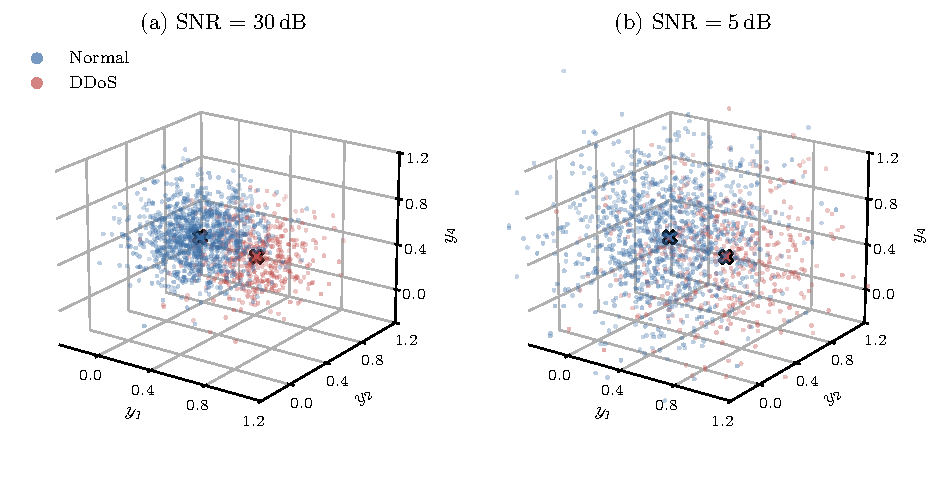
\includegraphics[width=\textwidth]{three_d_feature_space.pdf}
	\caption{Dreidimensionaler Ausschnitt des Merkmalsraums ($y_1$, $y_2$, $y_4$) für dieselben $1\,500$ Flüsse bei (a) $30$\,dB und (b) $5$\,dB. Blau: Normalverkehr, rot: DDoS, Kreuze: Klassenmittelwerte $\boldsymbol\mu_c$.}
	\label{fig:feature_raum_3d}
\end{figure}

Evaluiert werden $\mathrm{SNR}\in\{30,20,10,5\}$\,dB. Mehr zur technischen Umsetzung steht in Abschnitt~\ref{sec:gymnasium_umgebung} und~\ref{sec:awgn_kanal}.

\section{Umgang mit Klassenungleichgewichten (Imbalanced Data)}
\label{sec:imbalanced_data}

Ein wesentlicher methodischer Aspekt in der Erkennung von Netzwerkangriffen ist das Problem des Klassenungleichgewichts, auch als Imbalanced Data bezeichnet. In realen Netzwerken tritt der legitime Verkehr typischerweise deutlich häufiger auf als Angriffsverkehr, wodurch die Zielklassen in den Trainingsdaten stark asymmetrisch verteilt sind. Diese Verteilung ist in Sicherheitsanwendungen nicht nur statistisch relevant, sondern auch fachlich bedeutsam, da die Minderheitsklasse, also der bösartige Verkehr, häufig die operational entscheidenden Ereignisse repräsentiert. Ein Modell, das nur auf Gesamtgenauigkeit optimiert wird, kann daher eine hohe Gesamtleistung erzielen, zugleich aber die Erkennung von Angriffen vernachlässigen, weil die Mehrheitsklasse den Lernprozess dominiert.

Das Problem des Klassenungleichgewichts wirkt sich auf mehrere Ebenen aus. Zum einen entstehen im Training verzerrte Entscheidungsgrenzen, wenn der Algorithmus die Minderheitsklasse als wenig relevant behandelt. Zum anderen kann die Bewertung der Modelle durch klassische Metriken wie Accuracy irreführend werden, weil eine hohe Gesamtzahl korrekt klassifizierter Instanzen nicht zwingend einer guten Angriffserkennung entspricht. Gerade in einem Sicherheitskontext ist jedoch die Erkennung von tatsächlich vorhandenen Angriffen von hoher Bedeutung, da bereits ein einzelner unerkannter Angriff zu erheblichen Ausfallzeiten oder organisatorischen Schäden führen kann.

Für die Behandlung unbalancierter Datensätze stehen verschiedene Strategien zur Verfügung. Datenbasiert können Verfahren wie Oversampling, Undersampling oder synthetische Generierung von Minderheitsinstanzen angewendet werden, um die relative Repräsentation der Angriffs- und Normalverkehrsanteile anzupassen. Modellbasiert können zudem klassenspezifische Gewichte, kosten-sensitive Verlustfunktionen oder adaptierte Entscheidungsgrenzen eingesetzt werden, damit die Fehlklassifikation von Angriffen im Lernprozess stärker penalisiert wird. In dieser Arbeit liegt der Angriffsanteil bei $0{,}3$ und die Fehlerkosten werden über die Reward-Matrix gewichtet ($R_{FN}=-2$ gegenüber $R_{FP}=-1$), ohne Resampling. Eine methodisch saubere Anwendung von Resampling erfordert dabei, dass Resampling und Gewichtungen ausschließlich auf den Trainingsdaten erfolgen, um Datenleckage zu vermeiden und die spätere Evaluation auf repräsentativen Testdaten zu basieren.

Neben der Anpassung der Trainingsstrategie ist auch die Auswahl geeigneter Evaluationsmetriken von zentraler Bedeutung. Während Accuracy in unbalancierten Datensätzen nur eingeschränkt aussagekräftig ist, liefern Precision, Recall, F1-Score und im geeigneten Kontext auch ROC-AUC oder PR-AUC eine belastbarere Einschätzung der Erkennungsleistung. Diese Kennzahlen erlauben eine differenzierte Bewertung, ob ein Modell zwar viele legitime Verbindungen korrekt erkennt, aber zugleich die gefährlichsten Angriffsbeispiele verfehlt. Für die hier betrachtete Anwendung ist diese Unterscheidung von besonderer Bedeutung, da eine hohe Sensitivität bei der Angriffserkennung oft Vorrang vor einer rein hohen Gesamtgenauigkeit hat.

Insgesamt zeigt sich, dass die Behandlung von Klassenungleichgewichten nicht als isolierter Preprocessing-Schritt verstanden werden darf, sondern als integraler Bestandteil der gesamten Modell- und Evaluationspipeline. Erst durch eine konsistente Kombination aus geeigneter Datenrepräsentation, gezielter Feature-Auswahl, resampling-basierter Ausgewogenheit und aussagekräftiger Metrikbewertung lässt sich eine belastbare und praxisnahe Erkennung von Angriffen in realen Netzwerken erreichen. Dieses Kapitel bildet damit die methodische Grundlage für die anschließende Implementierung und die nachfolgenden experimentellen Evaluationen.
